\chapter{EXEMPLO DE CAPÍTULO}
\label{chapter:exemplo}

Neste capítulo apresenta-se uma classificação dos métodos de localização bidimensional de MS em redes de telefonia móvel celular. Esta classificação simplificada utiliza apenas três critérios: o método de cálculo, o grau de participação do MS no cálculo de posição e o número mínimo de setores requerido para estimar a localização do MS. Estes critérios constituem o conjunto mínimo necessário para permitir uma avaliação comparativa das diversas soluções de localização disponíveis atualmente. Há, contudo, diversas taxonomias mais abrangentes na literatura~\cite{LocationMethodsSurvey2007}~\cite{WlanLocationMethodsSurvey}~\cite{LocationMethodsSurvey2008}, não restritas a redes celulares, que utilizam esses e outros parâmetros para a classificação. Por exemplo, algumas taxonomias agrupam os métodos de localização em função do tipo de ambiente~(\textit{indoor} ou \textit{outdoor}) onde são aplicáveis~\cite{WlanLocationMethodsSurvey}. Esta divisão não é seguida aqui, pois diversos métodos, como os de correlação de assinaturas de rádio-frequência, identidade da célula, etc., podem ser aplicados em ambos os ambientes~\cite{DcmForGsm}.

\section{\textbf{Conceitos Básicos}}
\label{sec:Cap1Conceitos}

Alguns conceitos que serão utilizados na descrição dos métodos de localização precisam ser previamente definidos.

\subsection{\underline{Área Predita de Melhor Servidor de um Setor}}
É a área geográfica calculada por meio de um modelo de rádio-propagação onde o nível de sinal recebido~(RSS - \textit{Received Signal Strength}) predito do setor em questão é maior que o de qualquer outro setor da rede. A~\ref{fig:bestserverarea} ilustra as áreas preditas de melhor servidor de três setores de uma mesma BTS, calculadas aplicando o modelo de predição empírico de Okumura-Hata~\cite{HATA1980}. O relevo e os prédios são representados na base topográfica digitalizada da região. As perdas adicionais por difração sobre estes obstáculos foram calculadas por meio do modelo de Epstein-Peterson~\cite{MDY1993}.

\begin{figure}[H]
\begin{center}
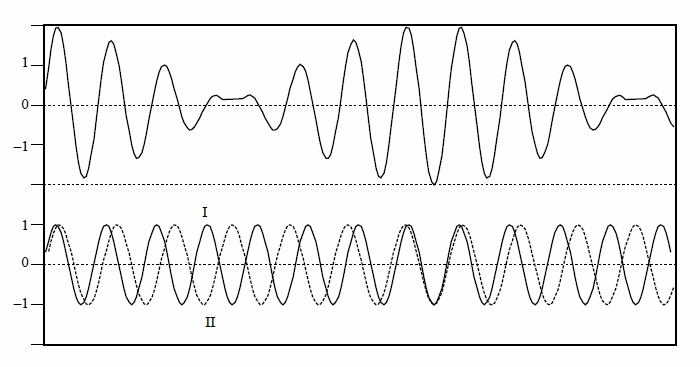
\includegraphics[width=8cm,height=6.4cm]{./02_Capitulos/02_Cap1/figures/fig_06_br.png}
\caption{\label{fig:bestserverarea}- Áreas Preditas de Melhor Servidor de Três Setores.}
\end{center}
\end{figure}

\section{\textbf{Classificação segundo o Método de Cálculo}}
\label{sec:Cap1Metodo}

O primeiro critério de classificação é a maneira pela qual os métodos de localização calculam a estimativa de posição do MS no plano. Para utilizar a geometria euclidiana, é necessário que as coordenadas geográficas dos setores de referência e do MS sejam representadas através uma projeção cartográfica retangular, ou seja, utilizando um sistema de coordenadas cartesianas. Os principais exemplos de sistemas de coordenadas retangulares utilizados em cartografia são o sistema UTM~(\textit{Universal Transverse Mercator})~\cite{Geocartografia}, que utiliza a projeção cartográfica transversa de Mercator, e o sistema MGRS~(\textit{Military Grid Reference System})~\cite{MGRS}.

\subsection{\underline{Identidade da Célula}}
\label{subsec:Cap1Cid}

No método de localização da identidade da célula~(CID - \textit{Cell Identity}), a posição do MS é assumida como sendo igual à da antena transmissora do setor melhor servidor. O método CID, embora seja de baixa complexidade e elevada disponibilidade, apresenta uma precisão muito dependente da densidade de setores na área de interesse~\cite{SPAWC2008}. Assim, o erro de localização pode variar de algumas centenas de metros em áreas urbanas até vários quilômetros em áreas rurais.

\subsection{\underline{Triangulação}}
\label{subsec:Cap1Triangulacao}

As técnicas de triangulação utilizam medidas de distâncias~(multi-lateração) ou ângulos~(multi-angulação) entre o MS e os setores de referência para estimar a localização do MS~\cite{LocationMethodsSurvey2007}.

Todos os métodos de triangulação presumem condições de propagação com linha de visada~(LOS - \textit{Line of Sight}) entre o MS e setores de referência. A propagação por múltiplos percursos e a presença de obstáculos entre o MS e os setores de referência podem corromper as medidas angulares, de tempo e de atenuação no percurso. Assim, a propagação sem linha de visada~(NLOS - \textit{Non Line of Sight}) é a principal fonte de erro para esses métodos. Como a propagação NLOS predomina em ambientes urbanos, a precisão dos métodos de triangulação pode ser seriamente comprometida nesses ambientes.

Além da propagação NLOS, outro fator que limita a precisão dos métodos de triangulação é a resolução finita das medidas realizadas na interface aérea e que são utilizadas no cálculo de posição: tempo, RSS e ângulo de chegada. A resolução da medida de RSS depende de especificações da interface rádio. Em redes GSM e WCDMA, por exemplo, os valores de RSS são reportados pelo MS em passos de $1$ dB~\cite{ETSI100911}~\cite{3GPP25133}. A resolução da medida angular depende da configuração dos conjuntos de antenas diretivas necessários para estimar o ângulo de chegada, bem como do diagrama de irradiação das antenas utilizadas no conjunto~\cite{Rappaport1997}.

\subsubsection{Multi-lateração Circular utilizando RTT}
Um valor de RTT pode ser convertido em uma estimativa de distância, através da equação~(\ref{eq:dist}). O lugar geométrico dos pontos que distam $\hat{d}_{i}$ da $i$-ésima célula de referência é um círculo de raio $\hat{d}_{i}$ centrado na posição desta célula. Esse círculo define o conjunto dos pontos no plano que contém a possível localização do MS, sendo denominado linha de posição (LOP - \textit{Line of Position}).

\begin{equation}
\label{eq:dist}
\hat{d}_{i}= \frac{c \cdot \textrm{T}_{s} \cdot \textrm{RTT}_{i}}{2}
\end{equation}

A medida de RTT tem resolução igual ao período de um símbolo. Porém, por razões de simplificação, utiliza-se a representação por meio de LOPs circulares, com raio igual ao raio interno no anel circular. Quanto menor o período de símbolo, menor é a largura do anel circular e mais este anel aproxima-se de um círculo. Assim, em sistemas banda larga, como o WCDMA, a utilização de LOPs circulares não introduz erro significativo~\cite{CidRttForcedHandover}.

\section{\textbf{Quadro Sinótico}}
\label{sec:Cap1Quadro}

A~\ref{tab:quadrosinotico} resume as principais características dos métodos de localização apresentados neste capítulo: o método de cálculo, a participação do MS no cálculo da posição, a quantidade mínima de setores requerida para calcular a posição do MS e os elementos adicionais necessários na rede de acesso rádio~(RAN - \textit{Radio Access Network}). A última coluna informa se o método depende de condições de propagação LOS entre o MS e as células de referência - ou os satélites, no caso do método AGPS - para não sofrer degradação da acurácia de localização.

Como a precisão de um método de localização é fortemente dependente das características específicas da rede onde o mesmo será utilizado - largura de banda, resolução temporal, densidade superficial de setores, ambiente de propagação, etc. - optou-se por não inserir na~\ref{tab:quadrosinotico} valores genéricos de precisão, como os fornecidos em~\cite{WlanLocationMethodsSurvey}.

\begin{table}[h]
\centering
\caption{\label{tab:quadrosinotico}- Quadro Sinótico dos Métodos de Localização.}
\vspace*{.1cm}
\begin{scriptsize}
\begin{tabular}{|c|c|c|c|c|c|}
\hline
\textbf{Sigla} & \textbf{Método de Cálculo} & \textbf{Participação} & \textbf{Quant. Mín.} & \textbf{Elem. adicionais} & \textbf{Requer}\\
& & \textbf{do MS} & \textbf{de Setores} & \textbf{na RAN} & \textbf{LOS ?}\\
\hline
AOA	& Triang. por multi-angulação & Baseado & 2	& Conj. de antenas & Sim \\
& & na Rede & & diretivas & \\
\hline
CID	& Identidade da célula	& Baseado & 1	& - & Não\\
& & na Rede & & & \\
\hline
EOTD	& Triang. por multi-lateração &	Assistido ou &	3	& LMUs & Sim \\
& hiperbólica & Baseado no MS & & & \\
\hline
AGPS	& Triang. por multi-lateração & Assistido & 3 & - & Sim \\
& circular & pelo MS & & & \\
\hline
CID+RTT	& Triang. por multi-lateração &	Baseado & 3	& - & Sim \\
& circular com RTT & na Rede & & & \\
\hline
CID+RSS	& Triang. por multi-lateração circular  &	Baseado & 3	& - & Sim \\
& com perda de propagação & na Rede & & & \\
\hline
AOA+RTT	& Híbrido	& Baseado & 1	&  Conj. de antenas & Sim \\
& & na Rede & & diretivas & \\
\hline
AOA+RSS	& Híbrido	& Baseado & 1	&  Conj. de antenas & Sim \\
& & na Rede & & diretivas& \\
\hline
AOA+TDOA	& Híbrido	& Assistido & 2	&  Conj. de antenas & Sim \\
& & pelo MS & & diretivas& \\
\hline
\end{tabular}
\end{scriptsize}
\vspace*{-.2cm}
\end{table}
